\section{Theorie\footnote{Unter Verwendung der Quelle \cite{Versuchsanleitung}.}}
\label{sec:Theorie}

\subsection{Einleitung}

Im folgenden Experiment soll das Relaxationsverhalten eines RC-Kreises -- also einer Reihenschaltung aus einem ohmschen 
Widerstand $R$ und einem Kondensator der Kapazität $C$, die mit einer Spannungsquelle verbunden sind -- untersucht werden. 
Sowohl Gleichspannung als auch verschiedene Wechselspannungsformen sind hinsichtlich ihres Einflusses auf die Ladevorgänge 
des Kondensators von Interesse für den Versuch.

\subsection{Auf- und Entladen von Kondensatoren bei Gleichspannung}
\label{sub:AufUndAb}

\begin{figure}
    \centering
    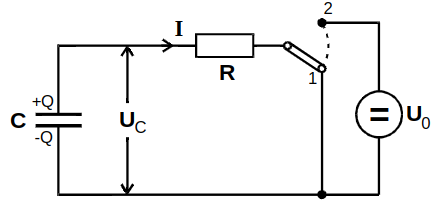
\includegraphics[width=0.8\textwidth]{plots/Schaltung1.png}
    \caption{Ein typischer RC-Kreis.}
    \label{fig:stinknormal_RC}
\end{figure}

In Abbildung \ref{fig:stinknormal_RC} ist ein typischer RC-Kreis zu sehen. 
Eine Gleichspannung $U_0$ kann den Kondensator über den Widerstand aufladen, wenn der Schalter in Position 2 ist. 
Entladen wird er, wenn Schalterposition 1 benutzt wird. 
Hier und im Folgenden wird die am Kondensator anliegende, der Speisespannung entgegengesetzten Spannung durch den  
Variablennamen $U_C(t)$ dargestellt. 

Um einen quantitativen Zusammenhang zwischen den Größen herzustellen, werden die Kirchhoff'schen Gesetze angewendet: 
\begin{equation}
    U_0 = RI(t)+U_C(t)
    \label{eqn:nummeroeins}
\end{equation}
Der Strom $I(t)$ entspricht der Ladungsänderung $\dot{Q}(t)$ auf den Kondensatorplatten, außerdem definiert sich die 
Kapazität eines Kondensators über ${C=\sfrac{Q}{U_C}}$. 
Durch Einsetzen in \eqref{eqn:nummeroeins} ergibt sich die Differentialgleichung 
\begin{equation}
    \dot{U}_C(t) + \frac{1}{RC}U_C(t) = \frac{1}{RC}U_0\,,
    \label{eqn:DGL1}
\end{equation}
die sich mit dem Ansatz 
\begin{equation}
    \int_{U_C(0)}^{U_C(t)} \frac{RC}{U_0 - U_C} \, \symup{d} U_C = \int_0^t \, \symup{d}t
    \label{eqn:DGL1_solu}
\end{equation}
lösen lässt zu 
\begin{equation}
    U_C(t)=U_0 + (U_C(0)-U_0)\symup{e}^{\frac{-t}{RC}} \, . 
    \label{eqn:U_C_DC}
\end{equation}

Das Aufladen geschieht demnach gemäß
\begin{equation}
    U_C(t)=U_0(1-\symup{e}^{\frac{-t}{RC}})\, .
    \label{eqn:upload}
\end{equation}
Die Differentialgleichung des Entladevorgangs besitzt keine Inhomogenität wie \eqref{eqn:DGL1}, unterscheidet sich abgesehen 
davon aber nicht. 
Sie wird erfüllt durch die Gleichung 
\begin{equation}
    U_C(t)=U_C(0)\symup{e}^{\frac{-t}{RC}} \,.
    \label{eqn:download}
\end{equation}
Beiden Lösungstermen ist die Zeitkonstante ${\tau=RC}$ gemein, die konventionellerweise eine Kenngröße des jeweiligen 
RC-Kreises darstellt: Nach einer Zeit von ${t=\tau}$ hat sich die jeweilig zu betrachtende Größe um etwa $63.2\%$ ihrem Langzeitzustand 
angenähert. 
\FloatBarrier

\subsection{Einfluss der Wechselspannung auf Amplitude und Phasenverschiebung}

Wird nun eine periodische Wechselspannung der Form $U(t)=U_0\cos(\omega t)$ angelegt, bekommt die Differentialgleichung 
eine entsprechende periodische Inhomogenität:
\begin{equation}
    \dot{U}_C(t) + \frac{1}{RC}U_C(t) = \frac{1}{RC}U_0 \cos(\omega t)\,.
    \label{eqn:DGL2}
\end{equation}
Da hier ausschließlich der Fall betrachtet wird, dass der Kondensator am Anfang ungeladen ist, ist die homogene Lösung 
$U_{C\text{,hom}}(t)=A\exp(\sfrac{-t}{RC})$ an dieser Stelle nicht relevant (weil ${A=0}$). 
Wird der Ansatz der rechten Seite ${U_C(t)=D\sin(\omega t) + E\cos(\omega t)}$ in \eqref{eqn:DGL2} eingesetzt, ergeben sich folgende Umformungen: 
\begin{equation}
    \stackrel{\text{in \eqref{eqn:DGL2}}}{\to} \omega D\cos(\omega t)-\omega E\sin(\omega t) + 
    \frac{D}{RC}\sin(\omega t) + \frac{E}{RC}\cos(\omega t) \stackrel{!}{=} \frac{U_0}{RC}\cos(\omega t)
\end{equation}
\begin{equation}
    \Leftrightarrow D=RC\omega E \quad \land \quad
    \omega D + \frac{E}{RC} = \frac{U_0}{RC}
\end{equation}
\begin{equation}
    \Leftrightarrow E=\frac{U_0}{1+\omega^2R^2C^2} \quad \land \quad D=\frac{RC\omega U_0}{1+\omega^2R^2C^2}
\end{equation}
\begin{equation}
    D\sin x + E\cos x = F\cos(x+\varphi)
\end{equation}
\begin{gather}
    \Leftrightarrow \varphi=\arctan(\frac{-D}{E}) = \arctan(-RC\omega)  \\
    \land F=\sqrt{D^2+E^2}=E\sqrt{1+R^2C^2\omega^2}
\end{gather}
Die Lösungsfunktion der Kondensatorspannung hat also die Form 
\begin{equation}
    U_C(t)=F(\omega)\cos(\omega t +\varphi(\omega))
    \label{eqn:U_C_AC}
\end{equation}
mit der frequenzabhängigen Amplitude und Phasendifferenz:
\begin{equation}
    F(\omega)=\frac{U_0}{\sqrt{1+R^2C^2\omega ^2}}
    \label{eqn:ampl_omega}
\end{equation}
\begin{equation}
    \varphi(\omega)=\arctan(-RC\omega)
    \label{eqn:phas_diff_omega}
\end{equation}
Die Phasendifferenz verschwindet für ${\omega \to 0}$, beträgt $\sfrac{\pi}{4}$ für ${\omega=\sfrac{1}{RC}}$ und geht gegen 
$\sfrac{\pi}{2}$ für ${\omega \to \infty}$. 
Die Amplitude nimmt für ${\omega \to 0}$ den Amplitudenwert der Generatorspannung an -- also $U_0$ -- , verkleinert sich 
um den Faktor $\sfrac{1}{\sqrt{2}}$ für ${\omega = \sfrac{1}{RC}}$ und nähert sich mit wachsender Frequenz immer mehr der Null. 
Diese Eigenschaften können zum Filtern von bestimmten Frequenzen von Nutzen sein. 
\FloatBarrier

\subsection{Integration mithilfe eines RC-Kreises}
Wird eine Spannung mit sehr hoher Frequenz $\omega \gg \sfrac{1}{RC}$ angelegt, mutiert \eqref{eqn:DGL2} zu
\begin{equation}
    \frac{U(t)}{RC}=\frac{\symup{d}U_C(t)}{\symup{d}t} \,,
    \label{eqn:dgl_xyz}
\end{equation}
da unter genannten Voraussetzungen ${\lvert U_C\rvert\ll\lvert U_R\rvert}$ und ${\lvert U_C\rvert\ll\lvert U\rvert}$ gelten. 
Die Differentialgleichung \eqref{eqn:dgl_xyz} zu einem Lösungsansatz umgeformt ergibt 
\begin{equation}
    U_C(t)=\frac{1}{RC} \int_0^t U(t') \,\symup{d}t'\,,
\end{equation}
was die integrierende Eigenschaft eines RC-Kreises bei hinreichend großer Frequenz $\omega$ deutlich macht, die ebenfalls 
im Verlauf des Experiments untersucht werden soll. 